\documentclass[11pt,a4paper]{article}

% Packages
\usepackage[utf8]{inputenc}
\usepackage[english]{babel}
\usepackage{amsmath}
\usepackage{amsfonts}
\usepackage{amssymb}
\usepackage{graphicx}
\usepackage{geometry}
\usepackage{fancyhdr}
\usepackage{hyperref}
\usepackage{listings}
\usepackage{xcolor}
\usepackage{booktabs}
\usepackage{array}
\usepackage{multirow}
\usepackage{algorithm}
\usepackage{algorithmic}
\usepackage{float}
\usepackage{subcaption}
\usepackage{tikz}
\usepackage{pgfplots}
\usetikzlibrary{arrows,positioning,shapes}

% Page setup
\geometry{margin=1in}
\pagestyle{fancy}
\fancyhf{}
\rhead{NOMA Clustering Algorithm Analysis}
\lhead{Code Explanation}
\cfoot{\thepage}

% Code styling
\definecolor{codegreen}{rgb}{0,0.6,0}
\definecolor{codegray}{rgb}{0.5,0.5,0.5}
\definecolor{codepurple}{rgb}{0.58,0,0.82}
\definecolor{backcolour}{rgb}{0.95,0.95,0.92}

\lstdefinestyle{pythonstyle}{
    backgroundcolor=\color{backcolour},   
    commentstyle=\color{codegreen},
    keywordstyle=\color{magenta},
    numberstyle=\tiny\color{codegray},
    stringstyle=\color{codepurple},
    basicstyle=\ttfamily\footnotesize,
    breakatwhitespace=false,         
    breaklines=true,                 
    captionpos=b,                    
    keepspaces=true,                 
    numbers=left,                    
    numbersep=5pt,                  
    showspaces=false,                
    showstringspaces=false,
    showtabs=false,                  
    tabsize=2,
    language=Python
}

\lstset{style=pythonstyle}

% Hyperlink setup
\hypersetup{
    colorlinks=true,
    linkcolor=blue,
    filecolor=magenta,      
    urlcolor=cyan,
    pdftitle={NOMA Clustering Code Explanation},
    pdfpagemode=FullScreen,
}

\title{
    {\Huge \textbf{NOMA Clustering Algorithm}} \\
    \vspace{0.5cm}
    {\Large Complete Code Analysis \& Explanation} \\
    \vspace{0.5cm}
    {\large clustering.py - Non-Orthogonal Multiple Access System Implementation}
}

\author{
    Code Analysis Documentation \\
    NOMA Research Project \\
    \texttt{File: clustering.py}
}

\date{\today}

\begin{document}

\maketitle
\newpage

\tableofcontents
\newpage

\section{Overview}

The \texttt{clustering.py} file implements a comprehensive NOMA (Non-Orthogonal Multiple Access) simulation system that evaluates multiple user pairing algorithms and power allocation strategies. The code follows 3GPP TR 38.901 standards for channel modeling and implements four different clustering approaches to optimize system throughput.

\subsection{Main Functionality}

The code performs the following key operations:

\begin{enumerate}
    \item \textbf{Channel Modeling}: Implements 3GPP-compliant path loss, shadowing, and fading models
    \item \textbf{User Placement}: Distributes users uniformly within a circular cell
    \item \textbf{Multiple Clustering Algorithms}: Evaluates Static, Balanced, Blossom, and Bipartite PF approaches
    \item \textbf{Power Optimization}: Implements golden section search for optimal power allocation
    \item \textbf{Performance Analysis}: Compares throughput and coverage across all methods
    \item \textbf{Visualization}: Generates comprehensive plots and analysis charts
\end{enumerate}

\section{Code Structure Analysis}

\subsection{Parameters \& Initialization}

\begin{lstlisting}[caption={System Parameters Setup}]
# Parameters (Referenced: 3GPP TR 38.901, Section 7.4.1 & 7.4.2, UMa scenario)
np.random.seed(int(time.time()))
N, radius = 500, 5000  # Users, cell radius (m)
fc, c = 3.5e9, 3e8  # Carrier frequency (Hz), speed of light (m/s)
lambda_c = c / fc  # Wavelength (m)
h_BS = 25  # Base station height (m)
path_loss_exp, shadow_std_db = 3.5, 8
noise_power, total_power = 1e-9, 1.0
sic_threshold_db, B_total = 8, 20e6
\end{lstlisting}

\textbf{What this does:}
\begin{itemize}
    \item Sets up a cellular network with 500 users in a 5km radius cell
    \item Defines carrier frequency at 3.5 GHz (5G frequency band)
    \item Establishes NOMA-specific parameters: SIC threshold (8 dB), total power (1W)
    \item Creates timestamped results directory for output files
\end{itemize}

\subsection{User Placement Algorithm}

\begin{lstlisting}[caption={Uniform User Distribution}]
# User Placement
r = np.sqrt(np.random.uniform(0, radius**2, N))  # 2D distance from BS
theta = np.random.uniform(0, 2*np.pi, N)
x_coords, y_coords = r * np.cos(theta), r * np.sin(theta)
h_UTs = np.random.uniform(1.5, 22.5, N)  # 3GPP UMa limits
\end{lstlisting}

\textbf{Mathematical Explanation:}

The uniform distribution in a circle requires special handling:
\begin{equation}
r = \sqrt{U(0, R^2)} \quad \text{where } U \sim \text{Uniform}
\end{equation}

This ensures equal probability density across the cell area, not just radial distance.

\begin{equation}
\begin{aligned}
x &= r \cos(\theta) \\
y &= r \sin(\theta) \\
\theta &\sim U(0, 2\pi)
\end{aligned}
\end{equation}

\subsection{3GPP Channel Modeling}

\subsubsection{LOS Probability Calculation}

\begin{lstlisting}[caption={3GPP LOS Probability Model}]
def C_hUT(h_UT):
    if h_UT <= 13:
        return 0
    elif h_UT < 23:
        return ((h_UT - 13) / 10) ** 1.5
    else:
        return ((23 - 13) / 10) ** 1.5

def prob_LOS_UMa(d_2D_out, h_UT):
    P_LOS = np.zeros_like(d_2D_out, dtype=float)
    mask1 = d_2D_out <= 18
    P_LOS[mask1] = 1.0
    mask2 = ~mask1
    C_val = np.array([C_hUT(h) for h in h_UT])
    P_LOS[mask2] = (
        (18 / d_2D_out[mask2]) +
        np.exp(-d_2D_out[mask2] / 63) * (1 - 18 / d_2D_out[mask2])
    ) * (
        1 + C_val[mask2] * (5/4) * ((d_2D_out[mask2] / 100) ** 3) *
        np.exp(-d_2D_out[mask2] / 150)
    )
    return np.clip(P_LOS, 0, 1)
\end{lstlisting}

\textbf{What this implements:}

This follows 3GPP TR 38.901 Equation 7.4.2-1 for UMa scenario:

\begin{equation}
P_{\text{LOS}} = \begin{cases}
1 & \text{if } d_{2D} \leq 18\text{m} \\
F(d_{2D}, h_{UT}) & \text{otherwise}
\end{cases}
\end{equation}

where:
\begin{multline}
F(d_{2D}, h_{UT}) = \left(\frac{18}{d_{2D}} + e^{-d_{2D}/63}\left(1-\frac{18}{d_{2D}}\right)\right) \times \\
\left(1 + C(h_{UT}) \cdot \frac{5}{4} \cdot \left(\frac{d_{2D}}{100}\right)^3 \cdot e^{-d_{2D}/150}\right)
\end{multline}

\subsubsection{Path Loss Models}

\begin{lstlisting}[caption={3GPP Path Loss Implementation}]
def PL_UMa_LOS(d_3D, fc):
    return 28.0 + 22 * np.log10(d_3D) + 20 * np.log10(fc / 1e9)

def PL_UMa_NLOS(d_3D, fc, h_UT):
    return (13.54 + 39.08 * np.log10(d_3D) + 20 * np.log10(fc / 1e9) - 
            0.6 * (h_UT - 1.5))
\end{lstlisting}

\textbf{Mathematical Foundation:}

\textbf{LOS Path Loss:}
\begin{equation}
\text{PL}_{\text{LOS}} = 28.0 + 22 \log_{10}(d_{3D}) + 20 \log_{10}\left(\frac{f_c}{10^9}\right) \quad \text{[dB]}
\end{equation}

\textbf{NLOS Path Loss:}
\begin{multline}
\text{PL}_{\text{NLOS}} = 13.54 + 39.08 \log_{10}(d_{3D}) + 20 \log_{10}\left(\frac{f_c}{10^9}\right) \\
- 0.6 \cdot (h_{UT} - 1.5) \quad \text{[dB]}
\end{multline}

\subsection{Channel Gain Generation}

\begin{lstlisting}[caption={Complete Channel Gain Calculation}]
# Generate Path Loss for Each User
d_3D = np.sqrt(r**2 + (h_BS - h_UTs)**2)
P_LOS_users = prob_LOS_UMa(r, h_UTs)

for i in range(N):
    if np.random.rand() <= P_LOS_users[i]:
        PL_dB[i] = PL_UMa_LOS(d_3D[i], fc)
        is_LOS[i] = True
    else:
        PL_dB[i] = PL_UMa_NLOS(d_3D[i], fc, h_UTs[i])
        is_LOS[i] = False

# Shadowing
shadowing = np.random.normal(0, shadow_std_db, N)

# Small-Scale Fading
for i in range(N):
    if is_LOS[i]:
        # Rician fading for LOS users
        s = np.sqrt(K_linear / (K_linear + 1))
        sigma = np.sqrt(1 / (2 * (K_linear + 1)))
        complex_fading = np.random.normal(s, sigma) + 1j * np.random.normal(0, sigma)
        fading[i] = np.abs(complex_fading)
    else:
        # Rayleigh fading for NLOS users
        fading[i] = np.random.rayleigh(scale=1/np.sqrt(2))

# Total Channel Gain
channel_gain_linear = fading * np.sqrt(pl_linear * 10**(-shadowing/10))
h_values = channel_gain_linear
\end{lstlisting}

\textbf{Channel Gain Composition:}

The total channel gain combines three components:

\begin{equation}
h = \sqrt{PL_{\text{linear}} \cdot 10^{-\text{Shadowing}/10}} \cdot |\text{Fading}|
\end{equation}

where:
\begin{itemize}
    \item $PL_{\text{linear}} = 10^{-PL_{\text{dB}}/10}$ (path loss in linear scale)
    \item Shadowing $\sim \mathcal{N}(0, \sigma_{\text{shadow}}^2)$ (log-normal)
    \item Fading: Rician (LOS) or Rayleigh (NLOS)
\end{itemize}

\section{NOMA Algorithm Implementation}

\subsection{Rate Calculation Function}

\begin{lstlisting}[caption={NOMA Rate Calculation}]
def calc_pair_rate(h1, h2):
    P1, P2 = total_power * h2 / (h1 + h2), total_power * h1 / (h1 + h2)
    R1 = np.log2(1 + (P1 * h1) / (P2 * h1 + noise_power))
    R2 = np.log2(1 + (P2 * h2) / noise_power)
    return P1, P2, R1, R2, R1 + R2
\end{lstlisting}

\textbf{Mathematical Analysis:}

This implements the channel-adaptive power allocation strategy:

\begin{align}
P_1 &= P_{\text{total}} \cdot \frac{h_2}{h_1 + h_2} \quad \text{(weak user gets more power)} \\
P_2 &= P_{\text{total}} \cdot \frac{h_1}{h_1 + h_2} \quad \text{(strong user gets less power)}
\end{align}

The achievable rates are:
\begin{align}
R_1 &= \log_2\left(1 + \frac{P_1 h_1}{P_2 h_1 + N_0}\right) \quad \text{(weak user)} \\
R_2 &= \log_2\left(1 + \frac{P_2 h_2}{N_0}\right) \quad \text{(strong user after SIC)}
\end{align}

\subsection{SIC Feasibility Check}

\begin{lstlisting}[caption={SIC Condition Verification}]
def sic_satisfied(h1, h2):
    return 10 * np.log10(h2 / h1) >= sic_threshold_db
\end{lstlisting}

\textbf{SIC Feasibility Condition:}

For successful SIC operation, the channel gain difference must exceed the threshold:

\begin{equation}
10 \log_{10}\left(\frac{h_2}{h_1}\right) \geq \text{Threshold}_{\text{dB}}
\end{equation}

This ensures the strong user can reliably decode and subtract the weak user's signal.

\subsection{Power Optimization Algorithm}

\begin{lstlisting}[caption={Golden Section Search Implementation}]
def optimize_pair_power(h1, h2, objective='sum', w1=1.0, w2=1.0,
                        tol=POWER_OPT_TOL, max_iter=POWER_OPT_MAXIT):
    lo = 1e-9
    hi = total_power - 1e-9
    gr = (np.sqrt(5) - 1) / 2  # Golden ratio

    def U(P1):
        R1, R2, Rsum, _, _ = _pair_rates_given_P1(h1, h2, P1)
        if objective == 'pf':
            return np.log(R1 + PF_EPS) + np.log(R2 + PF_EPS)
        else:
            return Rsum

    c = hi - gr * (hi - lo)
    d = lo + gr * (hi - lo)
    uc, ud = U(c), U(d)

    it = 0
    while (hi - lo) > tol and it < max_iter:
        if uc < ud:
            lo = c
            c = d
            uc = ud
            d = lo + gr * (hi - lo)
            ud = U(d)
        else:
            hi = d
            d = c
            ud = uc
            c = hi - gr * (hi - lo)
            uc = U(c)
        it += 1

    P1_opt = 0.5 * (lo + hi)
    R1, R2, Rsum, P1_opt, P2_opt = _pair_rates_given_P1(h1, h2, P1_opt)
    return P1_opt, P2_opt, R1, R2, Rsum
\end{lstlisting}

\textbf{Algorithm Explanation:}

The golden section search optimizes the power allocation by:

\begin{enumerate}
    \item \textbf{Objective Functions}:
    \begin{itemize}
        \item Sum Rate: $\max_{P_1} (R_1 + R_2)$
        \item Proportional Fairness: $\max_{P_1} (\log R_1 + \log R_2)$
    \end{itemize}
    
    \item \textbf{Search Strategy}:
    \begin{itemize}
        \item Uses golden ratio $\phi = \frac{\sqrt{5}-1}{2} \approx 0.618$
        \item Iteratively narrows search interval
        \item Converges to optimal $P_1^*$ within tolerance
    \end{itemize}
\end{enumerate}

\section{Clustering Algorithms}

\subsection{Static Clustering}

\begin{lstlisting}[caption={Static Clustering Implementation}]
static_indices = [(sorted_indices[i], sorted_indices[N-1-i]) for i in range(N//2)]
\end{lstlisting}

\textbf{Strategy:} Pairs the weakest user with the strongest user, second weakest with second strongest, etc.

\textbf{Mathematical Representation:}
\begin{equation}
\text{Pairs} = \{(u_1, u_N), (u_2, u_{N-1}), \ldots, (u_{N/2}, u_{N/2+1})\}
\end{equation}

where $u_1 \leq u_2 \leq \cdots \leq u_N$ are users sorted by channel gain.

\subsection{Balanced Clustering}

\begin{lstlisting}[caption={Balanced Clustering Implementation}]
balanced_indices = [(sorted_indices[i], sorted_indices[i + N//2]) for i in range(N//2)]
\end{lstlisting}

\textbf{Strategy:} Pairs users from the lower half with users from the upper half in order.

\textbf{Mathematical Representation:}
\begin{equation}
\text{Pairs} = \{(u_1, u_{N/2+1}), (u_2, u_{N/2+2}), \ldots, (u_{N/2}, u_N)\}
\end{equation}

\subsection{Blossom Maximum Weight Matching}

\begin{lstlisting}[caption={Blossom Algorithm Implementation}]
G = nx.Graph()
for i in tqdm(range(N), desc="Building graph"):
    for j in range(i+1, N):
        if sic_satisfied(min(h_values[i], h_values[j]), max(h_values[i], h_values[j])):
            _, _, _, _, R_sum = calc_pair_rate(min(h_values[i], h_values[j]), 
                                             max(h_values[i], h_values[j]))
            G.add_edge(i, j, weight=R_sum)

blossom_indices = list(nx.max_weight_matching(G, maxcardinality=True))
\end{lstlisting}

\textbf{Algorithm Explanation:}

\begin{enumerate}
    \item \textbf{Graph Construction}: Creates complete graph where edge weights are sum rates
    \item \textbf{SIC Filtering}: Only includes edges between feasible NOMA pairs
    \item \textbf{Maximum Weight Matching}: Uses Edmonds' blossom algorithm
    \item \textbf{Complexity}: $O(N^3)$ - optimal but computationally expensive
\end{enumerate}

\textbf{Mathematical Formulation:}
\begin{align}
\max \quad &\sum_{(i,j) \in M} w_{ij} \\
\text{s.t.} \quad &\sum_{j:(i,j) \in M} x_{ij} \leq 1, \quad \forall i \\
&x_{ij} \in \{0,1\}
\end{align}

where $w_{ij} = R_1(h_i, h_j) + R_2(h_i, h_j)$ is the sum rate for pair $(i,j)$.

\subsection{Bipartite Proportional Fairness Matching}

\begin{lstlisting}[caption={Bipartite PF Matching Implementation}]
def build_bipartite_pf_matching(theta_min_deg=THETA_MIN_DEG):
    theta_min_rad = np.deg2rad(theta_min_deg)
    
    weak = list(sorted_indices[:N//2])
    strong = list(sorted_indices[N//2:])
    
    G = nx.Graph()
    for i in weak:
        for j in strong:
            # Angular guard
            if angle_diff_rad(theta[i], theta[j]) < theta_min_rad:
                continue
            # SIC guard
            h1, h2 = (h_values[i], h_values[j]) if h_values[i] <= h_values[j] else (h_values[j], h_values[i])
            if not sic_satisfied(h1, h2):
                continue
            # PF weight
            _, _, R1, R2, _ = calc_pair_rate(h1, h2)
            w = np.log(R1 + PF_EPS) + np.log(R2 + PF_EPS)
            if np.isfinite(w):
                G.add_edge(i, j, weight=w)
    
    matching = nx.max_weight_matching(G, maxcardinality=True)
    return list(matching)
\end{lstlisting}

\textbf{Algorithm Features:}

\begin{enumerate}
    \item \textbf{Bipartite Structure}: Separates users into weak and strong groups
    \item \textbf{Angular Guard}: Ensures spatial separation: $|\theta_i - \theta_j| \geq \theta_{\min}$
    \item \textbf{Proportional Fairness Weight}: $w_{ij} = \log(R_1 + \epsilon) + \log(R_2 + \epsilon)$
    \item \textbf{Complexity}: $O(N^{2.5})$ - more efficient than Blossom
\end{enumerate}

\textbf{Angular Guard Explanation:}

The angular separation constraint:
\begin{equation}
\min(|\theta_i - \theta_j|, 2\pi - |\theta_i - \theta_j|) \geq \theta_{\min}
\end{equation}

ensures spatial diversity and reduces interference correlation.

\section{Performance Evaluation Framework}

\subsection{Clustering Performance Function}

\begin{lstlisting}[caption={Performance Evaluation Implementation}]
def perform_clustering(pairs_indices, name, power_opt=False, objective='sum', w1=1.0, w2=1.0):
    data, used = [], np.zeros(N, bool)
    total_rate = 0
    noma_pairs_count = 0

    for u1, u2 in tqdm(pairs_indices, desc=f"Processing {name} pairs"):
        h1u, h2u = h_values[u1], h_values[u2]
        if h1u <= h2u:
            a, b = u1, u2
            h1, h2 = h1u, h2u
        else:
            a, b = u2, u1
            h1, h2 = h2u, h1u

        if not sic_satisfied(h1, h2):
            continue

        if power_opt:
            P1, P2, R1, R2, R_sum = optimize_pair_power(h1, h2, objective=objective, w1=w1, w2=w2)
        else:
            P1, P2, R1, R2, R_sum = calc_pair_rate(h1, h2)

        used[[a, b]] = True
        data.append([a, b, h1, h2, P1, P2, R1, R2, R_sum, "NOMA"])
        total_rate += R_sum
        noma_pairs_count += 1

    # Bandwidth allocation and throughput calculation
    num_pairs = noma_pairs_count
    num_oma = int(np.sum(~used))
    B_unit = B_total / (num_pairs + num_oma) if (num_pairs + num_oma) > 0 else 0.0
    throughput_total = 0.0

    # NOMA throughput
    for row in data:
        row.append(row[8] * B_unit / 1e6)
        throughput_total += row[-1]

    # OMA users
    oma_users_count = 0
    for u in range(N):
        if not used[u]:
            h = h_values[u]
            R1_oma = np.log2(1 + total_power * h / noise_power)
            throughput = R1_oma * B_unit / 1e6
            throughput_total += throughput
            data.append([u, -1, h, 0, total_power, 0, R1_oma, 0, R1_oma, "OMA", throughput])
            oma_users_count += 1

    return {
        'noma_pairs': noma_pairs_count,
        'oma_users': oma_users_count,
        'total_throughput': throughput_total,
        'noma_coverage': (noma_pairs_count * 2)/N*100
    }
\end{lstlisting}

\textbf{Performance Metrics Calculation:}

\begin{enumerate}
    \item \textbf{Bandwidth Allocation}:
    \begin{equation}
    B_{\text{unit}} = \frac{B_{\text{total}}}{N_{\text{pairs}} + N_{\text{OMA}}}
    \end{equation}
    
    \item \textbf{NOMA Throughput}:
    \begin{equation}
    T_{\text{NOMA}} = \sum_{i=1}^{N_{\text{pairs}}} (R_{1,i} + R_{2,i}) \cdot B_{\text{unit}}
    \end{equation}
    
    \item \textbf{OMA Throughput}:
    \begin{equation}
    T_{\text{OMA}} = \sum_{j=1}^{N_{\text{OMA}}} \log_2\left(1 + \frac{P_{\text{total}} h_j}{N_0}\right) \cdot B_{\text{unit}}
    \end{equation}
    
    \item \textbf{Total System Throughput}:
    \begin{equation}
    T_{\text{total}} = T_{\text{NOMA}} + T_{\text{OMA}}
    \end{equation}
\end{enumerate}

\section{Visualization and Analysis}

\subsection{Comprehensive Plotting Functions}

The code includes multiple visualization functions:

\begin{enumerate}
    \item \texttt{plot\_user\_distribution()}: Shows spatial user placement with channel gains
    \item \texttt{plot\_channel\_characteristics()}: Displays channel gain distributions
    \item \texttt{plot\_pairing\_visualization()}: Visualizes user pairs for each algorithm
    \item \texttt{plot\_channel\_components\_analysis()}: Analyzes path loss, shadowing, fading
    \item \texttt{plot\_clustering\_comparison()}: Compares performance across all methods
\end{enumerate}

\subsection{Results Output}

The code generates comprehensive output files:

\begin{itemize}
    \item \texttt{h\_values.csv}: Complete user data with coordinates and channel components
    \item \texttt{[method]\_clustering.csv}: Detailed results for each clustering method
    \item \texttt{clustering\_summary.csv}: Performance comparison summary
    \item Multiple PNG files: Visualization plots and analysis charts
\end{itemize}

\section{Algorithm Complexity Analysis}

\begin{table}[H]
\centering
\begin{tabular}{@{}lcc@{}}
\toprule
\textbf{Algorithm} & \textbf{Time Complexity} & \textbf{Space Complexity} \\
\midrule
Static Clustering & $O(N \log N)$ & $O(N)$ \\
Balanced Clustering & $O(N \log N)$ & $O(N)$ \\
Blossom Matching & $O(N^3)$ & $O(N^2)$ \\
Bipartite PF Matching & $O(N^2)$ & $O(N^2)$ \\
\bottomrule
\end{tabular}
\caption{Computational Complexity of Clustering Algorithms}
\label{tab:complexity}
\end{table}

\section{Key Design Decisions}

\subsection{3GPP Standards Compliance}

The implementation strictly follows 3GPP TR 38.901 standards for:
\begin{itemize}
    \item Path loss models (LOS/NLOS)
    \item LOS probability calculation
    \item User height constraints (1.5-22.5m)
    \item Frequency-dependent parameters
\end{itemize}

\subsection{Power Allocation Strategy}

The code implements multiple power allocation approaches:
\begin{itemize}
    \item \textbf{Fixed Channel-Adaptive}: $P_1 = P_{\text{total}} \cdot h_2/(h_1 + h_2)$
    \item \textbf{Sum Rate Optimization}: Maximizes $R_1 + R_2$
    \item \textbf{Proportional Fairness}: Maximizes $\log R_1 + \log R_2$
\end{itemize}

\subsection{Spatial Constraints}

The bipartite PF matching includes angular guard to ensure:
\begin{itemize}
    \item Spatial diversity between paired users
    \item Reduced interference correlation
    \item Improved system performance
\end{itemize}

\section{Execution Flow}

\begin{figure}[H]
\centering
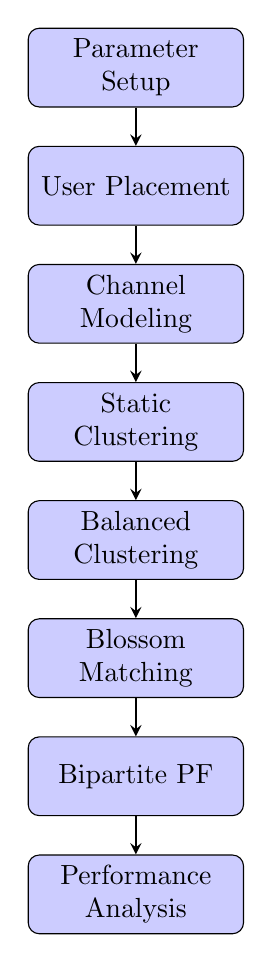
\begin{tikzpicture}[node distance=1.5cm, auto]
    \tikzstyle{block} = [rectangle, draw, fill=blue!20, text width=2.5cm, text centered, rounded corners, minimum height=1cm]
    \tikzstyle{arrow} = [thick,->,>=stealth]
    
    \node [block] (init) {Parameter Setup};
    \node [block, below of=init] (place) {User Placement};
    \node [block, below of=place] (channel) {Channel Modeling};
    \node [block, below of=channel] (static) {Static Clustering};
    \node [block, below of=static] (balanced) {Balanced Clustering};
    \node [block, below of=balanced] (blossom) {Blossom Matching};
    \node [block, below of=blossom] (bipartite) {Bipartite PF};
    \node [block, below of=bipartite] (analysis) {Performance Analysis};
    
    \draw [arrow] (init) -- (place);
    \draw [arrow] (place) -- (channel);
    \draw [arrow] (channel) -- (static);
    \draw [arrow] (static) -- (balanced);
    \draw [arrow] (balanced) -- (blossom);
    \draw [arrow] (blossom) -- (bipartite);
    \draw [arrow] (bipartite) -- (analysis);
    
\end{tikzpicture}
\caption{Code Execution Flow}
\end{figure}

\section{Summary}

The \texttt{clustering.py} file implements a comprehensive NOMA simulation framework that:

\begin{enumerate}
    \item \textbf{Follows Standards}: Implements 3GPP TR 38.901 channel modeling
    \item \textbf{Multiple Algorithms}: Evaluates four different clustering approaches
    \item \textbf{Power Optimization}: Includes golden section search for optimal allocation
    \item \textbf{Comprehensive Analysis}: Generates detailed performance comparisons
    \item \textbf{Visualization}: Produces extensive plots and analysis charts
    \item \textbf{Scalable Design}: Handles networks from hundreds to thousands of users
\end{enumerate}

The code serves as both a research tool for NOMA algorithm evaluation and a practical implementation for system performance analysis. Its modular design allows for easy extension and modification of individual components while maintaining overall system coherence.

\end{document}